\documentclass{article}

\usepackage[margin=1in]{geometry}
\usepackage{amsmath,amsthm,amssymb}
\usepackage{bbm, enumerate, tikz}
\usepackage{multicol}

\newenvironment{problem}[2][Problem]{\begin{trivlist}
\item[\hskip \labelsep {\bfseries #1}\hskip \labelsep {\bfseries #2.}]}{\end{trivlist}}
\newenvironment{note}[1][Note.]{\begin{trivlist}
\item[\hskip \labelsep {\bfseries #1}]}{\end{trivlist}}

\begin{document}

\title{Spring 2013: Complex Analysis Graduate Exam}
\author{Peter Kagey}

\maketitle

% -----------------------------------------------------
% First problem
% -----------------------------------------------------
\begin{problem}{1}
  Evaluate \[
    \int_0^\infty \frac{x^{1/3}}{1 + x^4}\,dx
  \] being careful to justify your answer.
\end{problem}

\begin{proof}
  For ease of notation, name the integrand $f$; that is, \[
    f(z) = \frac{z^{1/3}}{1 + z^4}.
  \]
  % Then $f$ has isolated singularities when $x^4 = e^{\pi i + 2\pi i k}$
  We will compute the integral by using the Residue Theorem together with (the
  limit of) the following contour:
  \begin{multicols}{2}
  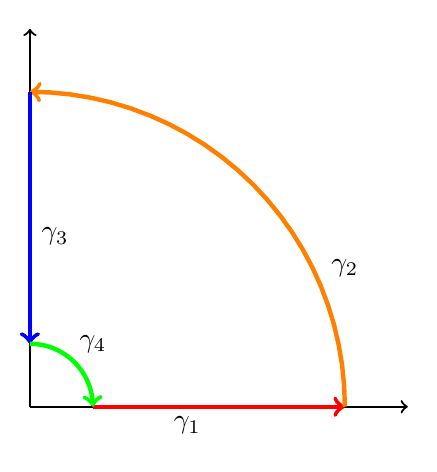
\begin{tikzpicture}[scale=0.8]
    % \draw[very thin,color=gray] (-0.9,-0.9) grid (5.9,5.9);
    \draw[thick, ->] (0,0)--(6,0);
    \draw[thick, ->] (0,0)--(0,6);
    \draw[ultra thick, ->, draw=red, domain=1:5] plot ({\x}, {0});
    \draw node at (2.5, -0.3) {$\gamma_{1}$};
    \draw[ultra thick, ->, draw=orange, domain=0:90] plot ({5*cos(\x)}, {5*sin(\x)});
    \draw node at (5, 2.2) {$\gamma_{2}$};
    \draw[ultra thick, <-, draw=blue, domain=1:5] plot ({0}, {\x});
    \draw node at (0.4, 2.7) {$\gamma_{3}$};
    \draw[ultra thick, ->, draw=green, domain=90:0] plot ({cos(\x)}, {sin(\x)});
    \draw node at (1, 1) {$\gamma_{4}$};
  \end{tikzpicture}\\
  \begin{align}
    \gamma_{1} &= \{t + 0i\ |\ t \in [\varepsilon, R] \} \\
    \gamma_{2} &= \{R e^{it}\ |\ t \in [0,\pi/2] \} \\
    \gamma_{3} &= \{0 + ti\ |\ t \in [\varepsilon, R]\} \\
    \gamma_{4} &= \{\varepsilon e^{it}\ |\ t \in [0, \pi/2]\}.
  \end{align}
  \end{multicols}
  For sufficiently small $\epsilon$ and large $R$, this contour encloses one
  singularity of $f$, namely $z_0 = e^{\pi i/4}$.
  \[
    \int_{\gamma_1} f(z)\,dz +
    \int_{\gamma_2} f(z)\,dz +
    \int_{\gamma_3} f(z)\,dz +
    \int_{\gamma_4} f(z)\,dz =
    2\pi i \operatorname{Res}_{z_0}(f).
  \]
  In the limit, both arcs ($\gamma_2$ and $\gamma_4$) vanish.
  \begin{align*}
    \left|\int_{\gamma_2}f(z)\,dz\right|
    &= \left|
      \int_0^{\pi/2}\frac{(Re^{it})^{1/3}}{1 + {(Re^{it})^4}}iRe^{it}\,dt
    \right|\\
    &\leq \int_0^{\pi/2}\left|
      \frac{(Re^{it})^{1/3}}{1 + {(Re^{it})^4}}iRe^{it}\,dt
    \right| \\
    &= \int_0^{\pi/2}\left|
      iR^{4/3}\frac{e^{4it/3}}{1 + {R^4e^{4it}}}\,dt
    \right| \\
    &\leq \int_0^{\pi/2}\left|
      iR^{4/3}\frac{e^{4it/3}}{{R^4e^{4it}}}\,dt
    \right| = \frac{\pi}{2}R^{-8/3}
  \end{align*} which vanishes as $R \rightarrow \infty$.
  Similarly, \begin{align*}
    \left|\int_{\gamma_4}f(z)\,dz\right|
    &= \left|
      \int_0^{\pi/2}\frac{(\varepsilon e^{it})^{1/3}}{1 + {(\varepsilon e^{it})^4}}i\varepsilon e^{it}\,dt
    \right|\\
    &\leq \int_0^{\pi/2}\left|
      \frac{(\varepsilon e^{it})^{1/3}}{1 + {(\varepsilon e^{it})^4}}i\varepsilon e^{it}\,dt
    \right| \\
    &= \int_0^{\pi/2}\left|
      i\varepsilon ^{4/3}\frac{e^{4it/3}}{1 + {\varepsilon ^4e^{4it}}}\,dt
    \right| \\
    &\leq \int_0^{\pi/2}\left|
      i\varepsilon ^{4/3}\frac{e^{4it/3}}{1}\,dt
    \right| = \frac{\pi}{2}\varepsilon ^{4/3}
  \end{align*} which also vanishes as $\varepsilon \rightarrow 0$.
  This means that our equation simplifies in the limit to \[
    \int_{\gamma_1} f(z)\,dz +
    \int_{\gamma_3} f(z)\,dz =
    2\pi i \operatorname{Res}_{z_0}(f).
  \] And the right hand side further simplifies to \begin{align*}
    \int_\varepsilon^R\frac{z^{1/3}}{1 + {z^4}}\,dz +
    \int_R^\varepsilon\frac{(iz)^{1/3}}{1 + {(iz)^4}}i\,dz &=
    \int_\varepsilon^R\frac{z^{1/3}}{1 + {z^4}}\,dz -
    i^{4/3}\int_\varepsilon^R\frac{z^{1/3}}{1 + {z^4}}\,dz\\
    &= (1 - i^{4/3}) \int_\varepsilon^R\frac{z^{1/3}}{1 + {z^4}}\,dz.
  \end{align*}
  So by the Residue Theorem, the integral evaluates to \[
    \int_\varepsilon^R\frac{z^{1/3}}{1 + {z^4}}\,dz
    = \frac{2\pi i\operatorname{Res}_{z_0}(f)}{1 - i^{4/3}}
    = \frac{2\pi i}{1 - e^{2\pi i/3}}\operatorname{Res}_{z_0}(f),
  \] and it is enough to compute the residue: \[
    \operatorname{Res}_{z_0}(f)
    = \frac{z_0^{1/3}}{(z_0^2 + i)(z_0 + z_0)}
    = \frac{e^{\pi i/12}}{(2e^{\pi i/2})(2e^{\pi i/4})}
    = \frac{1}{4} e^{-2\pi i/3}.
  \]
  Therefore \begin{align*}
    \int_\varepsilon^R\frac{z^{1/3}}{1 + {z^4}}\,dz
    &= \frac{2\pi i}{1 - e^{2\pi i/3}}\cdot\frac{1}{4} e^{-2\pi i/3}\\
    &= \frac{2\pi i}{1 - (-1/2 + \sqrt{3}i/2)}\cdot\frac{1}{4} e^{-2\pi i/3}\\
    &= \frac{4\pi i}{3 - \sqrt{3}i} \cdot\frac{1}{4}\left(-\frac{1}{2} - \frac{\sqrt{3}}{2}i\right)\\
    &= \frac{\pi}{3 - \sqrt{3}i} \cdot i\left(-\frac{1}{2} - \frac{\sqrt{3}}{2}i\right)\\
    &= \frac{\pi}{2} \left(\frac{\sqrt3-i}{3 - \sqrt{3}i}\right)\\
    &= \frac{\pi}{2\sqrt3}.
  \end{align*}
\end{proof}
% -----------------------------------------------------
% Second problem
% -----------------------------------------------------
\pagebreak

\begin{problem}{2}
  Assume that $f$ is an entire function such that \[
    |f(z)| \geq \frac{1}{1 + |z|}\ \text{for all}\ z \in \mathbb C.
  \] Prove that $f$ is a constant function.
\end{problem}

\begin{proof}
\end{proof}

% -----------------------------------------------------
% Third problem
% -----------------------------------------------------
\pagebreak

\begin{problem}{3}
  Let $f_n,\ n \geq 1$, be a sequence of holomorphic functions on an open
  connected set $D$ such that $|f_n(z)| \leq 1$ for all $z \in D,\ n \geq 1$.
  Let $A \subseteq D$ be the set of all $z \in D$ for which the limit
  $\lim_n f_n(z)$ exists.

  Show that if $A$ has an accumulation point in $D$, then there exists a
  holomorphic function $f$ on $D$ such that $f_n \rightarrow f$ uniformly on
  every compact set of $D$ as $n \rightarrow \infty$.
\end{problem}

\begin{proof}
\end{proof}

% -----------------------------------------------------
% Fourth problem
% -----------------------------------------------------
\pagebreak

\begin{problem}{4}
  Let $f(z)$ be meromorphic on $\mathbb C$, holomorphic for
  $\operatorname{Re} z > 0$ and such that $f(z + 1) = zf(z)$ in its domain with
  $f(1) = 1$.

  Show that $f$ has the first order poles at $0, -1, -2, \hdots$, and find the
  residues of $f$ at these points.
\end{problem}

\begin{proof}
  Notice first that inductively, we can write \[
    f(z)
    = \frac{f(z + 1)}{z}
    = \frac{\left(\frac{f(z + 2)}{z + 1}\right)}{z}
    = \frac{f(z + 2)}{z(z+1)}
    = \hdots
    = \frac{f(z + k + 1)}{z(z + 1)\cdots(z+k)}.
  \]
  Now, for each $k \in \mathbb N$, checking the limit \begin{align*}
    \lim_{z \rightarrow -k} (z + k)f(z)
    &= \lim_{z \rightarrow -k} (z + k)\frac{f(z + k + 1)}{z(z + 1)\cdots(z+k)} \\
    &= \lim_{z \rightarrow -k} \frac{f(z + k + 1)}{z(z + 1)\cdots(z+k-1)} \\
    &= \frac{f(1)}{(-k)(-k + 1)\cdots(-1)} \\
    &= \frac{(-1)^k}{k!}.
  \end{align*}
  Since this limit exists and is finite for all $k \in \mathbb N$, $f$ has first
  order poles at $-k$ for all $k$, and the residue of each pole is the value
  computed above: \[
    \operatorname{Res}_{-k}(f) = \frac{(-1)^k}{k!}.
  \]
\end{proof}

\end{document}
